%!TEX TS-program = lualatex
%!TEX encoding = UTF-8 Unicode

%\documentclass[t]{beamer}

%%%% HANDOUTS For online Uncomment the following four lines for handout
\documentclass[t,handout]{beamer}  %Use this for handouts.
\includeonlylecture{student}
\usepackage{handoutWithNotes}
\pgfpagesuselayout{3 on 1 with notes}[letterpaper,border shrink=5mm]
%	\setbeamercolor{background canvas}{bg=black!5}


%%% Including only some slides for students.
%%% Uncomment the following line. For the slides,
%%% use the labels shown below the command.

%% For students, use \lecture{student}{student}
%% For mine, use \lecture{instructor}{instructor}


%\usepackage{pgf,pgfpages}
%\pgfpagesuselayout{4 on 1}[letterpaper,border shrink=5mm]

% FONTS
\usepackage{fontspec}
\def\mainfont{Linux Biolinum O}
\setmainfont[Ligatures={Common,TeX}, BoldFont={* Bold}, ItalicFont={* Italic}, Numbers={Proportional}]{\mainfont}
\setsansfont[Scale=MatchLowercase]{Linux Biolinum O} 
\newfontface\lining[Numbers=Lining, Scale=MatchLowercase]{\mainfont}

\usepackage{microtype}

\usepackage{graphicx}
	\graphicspath{%
	{/Users/mtaylor/Pictures/teach/348/lectures/}%
	{/Users/mtaylor/Pictures/teach/common/}%}%
	{media_14/}} % set of paths to search for images

\usepackage{amsmath,amssymb}

%\usepackage{units}

\usepackage{booktabs}
\usepackage{multicol}
%	\setlength{\columnsep=1em}

\usepackage{array}
\newcolumntype{L}[1]{>{\raggedright\let\newline\\\arraybackslash\hspace{0pt}}p{#1}}
\newcolumntype{C}[1]{>{\centering\let\newline\\\arraybackslash\hspace{0pt}}p{#1}}
\newcolumntype{R}[1]{>{\raggedleft\let\newline\\\arraybackslash\hspace{0pt}}p{#1}}


\usepackage{tikz}
	\tikzstyle{every picture}+=[remember picture,overlay]
	\usetikzlibrary{arrows,calc}
	
\usepackage[version=4]{mhchem}
%\usepackage{siunitx}

%\usepackage{textcomp}
%\usepackage{setspace}
\mode<presentation>
{
  \usetheme{Lecture}
  \setbeamercovered{invisible}
  \setbeamertemplate{items}[square]
}

\usepackage{hyperref}

\newcommand\HiddenWord[1]{%
	\alt<handout>{\rule{4cm}{0.4pt}}{#1}%
}

\newcommand\skiptobottom{%
	\vskip0pt plus 1filll%
}

\begin{document}

\lecture{student}{student}

{
\setbeamercolor{background canvas}{bg=black}
\begin{frame}
  \includegraphics[width=\linewidth]{14_acid_test}
\end{frame}
}
\begin{frame}[t]{Historical temperatures were relatively steady until recently.}

	\vspace{-\baselineskip}

	{\centering
	\includegraphics[height=0.82\textheight]{14_historic_temps}\par}
	
	\vfilll
	
	\tiny \hfill Mann et al.~2008. PNAS 105: 13252.  
	
\end{frame}
%
\begin{frame}[t]{Global temperatures are increasing rapidly.}
	
	\includegraphics[width=0.49\linewidth]{14_holocene_temps1}
	\hfill
	\includegraphics[width=0.49\linewidth]{14_holocene_temps2}

	\vfilll

	\tiny Tamino 2013, modified Shakun et al. 2012\hfill Marcott et al. 2013
	
\end{frame}
%
\begin{frame}[b]{Holocene \ce{CO2} and pH will change rapidly.}

	\includegraphics[width=\linewidth]{14_co2_ph}
	
	\vfilll

	\hfill\tiny Nature.com/scitable: Ocean Acidification
	
\end{frame}
%
\begin{frame}[t]{How does the predicted future compare to the past for \ce{CO2} and pH?}

	{\centering\lining\begin{tabular}{@{}L{25mm}C{20mm}C{10mm}R{25mm}@{}}
		\toprule
		Time	&	p\ce{CO2}\newline (seawater) &	pH	&	[\ce{H+}] Increase (pre-industrial) \\
		\midrule
		Glacial	&	180	& 8.32	&	$-$30.8\% \\[1ex]
		Pre-Industrial	&	280	&	8.16	&	— \\[1ex]
		Present	&	380	&	8.05	&	$+$28.9\% \\[1ex]
		2 $\times$ \ce{CO2} (pre-industrial)	&	560	&	7.91	&	$+$77.7\% \\[1ex]
		3 $\times$ \ce{CO2} (pre-industrial) & 	840	& 7.76 & $+$151.4\% \\[1ex]
		\bottomrule
	\end{tabular}\par
	}

	\hangpara \highlight{Current atmospheric \ce{CO2} is sustained above 400 ppm!} 
	\vfilll

	\hfill \tiny Kleypas et al. 2006. NOAA Workshop Report.

\end{frame}
%

%
\begin{frame}[t]{Atmospheric [\ce{CO2}] determines ocean pH.}

	{\centering \ce{CO2 + H2O <-> H2CO3 <-> H+ + HCO3- <-> 2H+ + CO3^{2-}}\par
	}

	\vspace*{2\baselineskip}

	\hspace*{1em}\begin{tabular}{@{}ll@{}}
	[\ce{HCO3^-}] &	\textasciitilde90\% inorganic carbon \\[1em]
	[\ce{CO3^2-}] &	 \textasciitilde9\% inorganic carbon\\[1em]
	[\ce{CO2}] &	  \textasciitilde1\% inorganic carbon\\[1em]
	\end{tabular}

	\hangpara Current pH of ocean surface water: \textasciitilde8.05.

\end{frame}
%
%
\begin{frame}[t]{pH is maintained by the \highlight{bicarbonate buffering system.}}

	\includegraphics[width=0.98\textwidth]{14_carbonate_buffering_ratios_no_change}
	
	\begin{tikzpicture}
		\draw [blue] (20.9em,5.3em) -- node [right] {Current pH} (20.9em,20.2em);
	\end{tikzpicture}

	\vfilll
	
	\hfill \tiny BeAr, Wikimedia, public domain
\end{frame}
%
\begin{frame}{Increasing atmospheric [\ce{CO2}] increases ocean acidity.}

	\begin{center}
		\begin{tikzpicture}
	
			\alt<handout>{}{\only<1>{\node (equation) at (0,-1.5) {\ce{CO2 + H2O <-> H2CO3 <-> H+ + HCO3- <-> 2H+ + CO3^2-}};}}
			\only<2->{\node (equation) at (0,-1.5) {\ce{CO2 + H2O -> H2CO3 -> H+ + HCO3- <-> 2H+ + CO3^2-}};}

			\onslide<2->{\node (atmos) [left,align=left] at (0,0) {Increased atmospheric [\ce{CO2}]\\dissolves in ocean water,};
			\coordinate (eqpt1) at ($(equation.north west)!0.1!(equation.north)$);
			\coordinate (atmopt) at ($(atmos.south west)!0.2!(atmos.south)$);
			\draw [ultra thick, ->] (atmopt) -- (eqpt1);}
			
			
			\onslide<2->{\node (ocean) [right, align=left] at (0,-3) {which increases [\ce{H+}] and\\decreases ocean pH.};
				
			\draw [ultra thick, ->] (ocean.north west) -- (equation.south);}	
			
		\end{tikzpicture}
	\end{center}
	
\end{frame}
%
%
\begin{frame}{Increased [\ce{H+}] reduces availability of \ce{CO3^2-} to marine organisms.}

	\begin{center}
		\begin{tikzpicture}
	
			\node (excess) [right, align=left] at (-1,0) {Some excess [\ce{H+}] bonds with \ce{CO3^2-}};

			\node (equation) at (0,-1.5) {\ce{CO2 + H2O -> H2CO3 -> H+ + HCO3- <- 2H+ + CO3^2-}};

			\node (bicarb) [align=left] at (1,-3) {to form \ce{HCO3^-}};

			\coordinate (expt) at ($(excess.south east)!0.42!(excess.south)$);

			\coordinate (eqpt1) at ($(equation.north east)!0.28!(equation.north)$);

			\coordinate (eqpt2) at ($(equation.south)!0.21!(equation.south east)$);

			\draw [ultra thick, ->] (bicarb.north) -- (eqpt2);
				
			\draw [ultra thick, ->] (expt) -- (eqpt1);
			
		\end{tikzpicture}
	\end{center}

	\vspace*{7\baselineskip}
	
	\hangpara \highlight{Some \ce{H+} remains dissolved in water, lowering pH.}

\end{frame}
%
\begin{frame}[t]

	\includegraphics[width=\textwidth]{14_carbonate_buffering_ratios}
	
	\vfilll
	
	\hfill \tiny BeAr, Wikimedia, public domain
\end{frame}
%
\begin{frame}[t]{Carbonate availability depends on saturation state.}

	{\centering \ce{CaCO3 <-> Ca^2+ + CO3^2-}\par
	}

	\vspace*{\baselineskip}
	
\[ \Omega = \frac{[\ce{Ca^2+}][\ce{CO3^2-}]}{K_{\mathrm{sp}}^\prime} \]

%\[ \Omega = \ce{\frac{[Ca^2+][CO3^2-]}{K^\prime}_{\mathrm{sp}}} \]

	\vspace*{\baselineskip}

\hangpara $\Omega > 1 =$ shell and skeleton formation.\\

\hangpara $\Omega < 1 =$ shell and skeleton erosion.

\hangpara Increased [\ce{H+}] decreases $\Omega.$

\hangpara\highlight{Optimal $\Omega > 4.0.$}

\end{frame}
%
{
\usebackgroundtemplate{\includegraphics[width=\paperwidth]{14_carbonate_reduction}}
\begin{frame}[b]{[\ce{H+}] reduces available carbonate.}

\Tiny Hoegh-Guldberg et al. 2007. Science 318: 1737
\end{frame}
}
%
{
\usebackgroundtemplate{\includegraphics[width=\paperwidth]{14_aragonite_saturation_levels}}
\begin{frame}[b]

\hfill \tiny \rotatebox{90}{Kleypas et al. 2006. NOAA Workshop Report}
\end{frame}
}
%
\begin{frame}{Climate change causes ecological feedback.}
\includegraphics[width=\linewidth]{14_ecological_feedback}

\bigskip

{\small
Large arrows: impact points of acidification or warming. \\
Red lines: negative (decreasing) influence. \\
Green lines: positive (increasing) influence. \\
Rectangles: decreasing levels (dashed boxes may respond to local management). \\
Hexagons: increasing levels.}

\end{frame}
%
{
\usebackgroundtemplate{\includegraphics[width=\paperwidth]{14_alternate_stable_states}}
\begin{frame}[b]

	\hfill \tiny \rotatebox{90}{Hoegh-Guldberg et al. 2007. Science 318: 1737}
\end{frame}
}
%
{
\usebackgroundtemplate{\includegraphics[width=\paperwidth]{14_acidification_alternate_states}}
\begin{frame}[b]

	\hfill \tiny \rotatebox{90}{Hoegh-Guldberg et al. 2007. Science 318: 1737}
\end{frame}
}
%
\end{document}
